\documentclass{IEEEtran}
\usepackage[utf8]{inputenc} 
\usepackage[T1]{fontenc} 
\usepackage[turkish,shorthands=:!]{babel} 
\usepackage{hyperref}
\usepackage{graphicx}
\usepackage{minted}

\renewcommand\IEEEkeywordsname{Anahtar kelimeler}

\begin{document}

\title{3D Modelleme}
\author{Name1, No1, mail1 \\ Name2, No2, mail2 \\ Name3, No3, mail3} 

\markboth{PAÜ Bilgisayar Mühendisliği, CENG 104 - Bilgisayar Mühendisliği Semineri}{\@title} 


\maketitle

\begin{abstract}
Yapısal kalp hastalığı (SHD), kardiyovasküler tıpta yeni bir alandır. Geleneksel görüntüleme yöntemleri hastalık teşhisi kavramı etrafında yapılandırıldıkları için, SHD müdahalelerinin ihtiyaçlarını desteklemekde yetersiz kalmaktadır. SHD müdahaleler, görüntülemenin prosedür içi planlamasını, simülasyonunu ve tahmin edilmesini gerektiren geleneksel görüntüleme kavramlarını bozar. Transkateter SHD müdahalelerinde, altın standartta bir açık kavite cerrahi alanının olmaması, hekimleri dokunsal geri bildirim ve kardiyak anatominin görsel doğrulaması fırsatından mahrum eder. Bu nedenle, görüntülemeye bağımlılık prosedürel rehberlikte, yeni nesil prosedürel beceri setlerinin, görsel alan kavramının ve preklinik cihaz geliştirmeyi, hekimi için periprosedürel planlama döneminde teknolojiler kullanılır. Klinik bakım ve prosedür planlamasında 3 boyutlu (3D) baskının uyarlanması, transkateter müdahaleler için erken teşhiste önemlidir. Hesaplama modellemenin 3B'ye entegrasyonu baskı, cihaz testinde akışkanlar mekaniğinin araştırma ve geliştirme anlayışını hızlandırdı. 3D baskı, hesaplamalı modelleme ve nihayetinde yapay zekanın dahil edilmesi, sağlık uygulamalarının seyrini değiştiriyor. Transkateter yapısal kalp müdahaleleri derinlemesine incelenmeyi gerektirir. Geleneksel görüntüleme ile sağlanmayan kardiyak patofizyoloji ve cihaz etkileşimlerinin periprosedürel anlaşılması gerekmektedir. 
\end{abstract}

\begin{IEEEkeywords}
3D baskı, bilgisayarlı tomografi, hesaplamalı modelleme, sol atriyal uzantı, transkateter aort kapak değişimi, transkateter mitral kapak değişimi, transözofageal ekokardiyogram, yapay zeka, yapısal kalp hastalığı 
\end{IEEEkeywords}

\section{Giriş}
\label{sec:giris}
Bu doküman Pamukkale Üniversitesi Bilgisayar Mühendisliği Bölümü CENG 104 kodlu Bilgisayar Mühendisliği Semineri dersi için hazırlanan sunum dosyasıdır. Biçim olarak ``IEEE Transactions Journals and Conferences'' şablonu kullanılmıştır.

\section{3D BASKI, BİLGİSAYARLI MODELLEME VE AI'NIN TEMELLERİ}
\label{sec:3d}

\subsection{3D MODELLEME NEDİR?}
\label{subsec:nedir}

\subsection{3D BASKI TEKNOLOJİLERİNE GENEL BAKIŞ}
\label{subsec:genel}

\subsection{VERİ BÖLÜMLEME VE GÖRÜNTÜ OLUŞTURMA İLKELERİ}
\label{subsec:veri}

\section{YAPISAL KALP HASTALIKLARINDA 3D BASKI}
\label{sec:yapısal}

\subsection{TRANSKATETER AORTİK KAPAKÇIK DEĞİŞİMİ İÇİN 3D BASKI}
\label{subsec:aortik}

\subsection{TRANSKATETER MİTRAL KAPAKÇIK DEĞİŞİMİ İÇİN 3D BASKI VE SANAL SİMÜLASYON}
\label{subsec:mitral}

\subsection{TRANSKATETER TRİKÜSPİD KAPAKÇIK TAMİR VE DEĞİŞİMLERİ İÇİN 3D BASKI}
\label{subsec:tri}

\subsection{HASTA EĞİTİMİ}
\label{subsec:hasta}

\section{3D BASKININ GÜNCEL KISITLAMALARI}
\label{sec:yapısal}

\section{3D BASKININ ÖTESİNDE: BİLGİSAYARLI MODELLEME VE AI'NİN TEMELLERİ}
\label{sec:öte}

\section{YAPAY ZEKANIN SHD'DE ROLÜ}
\label{sec:ai}

\section{GİRİŞİMCİLERİN VE GİRİŞİMSEL GÖRÜNTÜLEME HEKİMLERİNİN EĞİTİMİ}
\label{sec:girişim}

\section{TEKNOLOJİDE AŞILMASI GEREKEN ZORLUKLAR}
\label{sec:tek}

\section{SONUÇ}
\label{sec:sonuc}

\section{KAYNAK}
\label{sec:kaynak}

\begin{table}
\caption{Doküman İçindeki Referans Tipleri}
\label{tab:referans}
\centering
\begin{tabular}{|l|c|} \hline
Referans tipi & Açıklama \\ \hline
sec: & section(bölüm) \\
subsec: & subsection(alt bölüm) \\
fig: & figure(şekil) \\
tab: & table(tablo) \\
\hline
\end{tabular}
\end{table}

\subsection{Kaynaklar}
\begin{itemize}
 \item Makale: \cite{ELSEVIER}
\end{itemize}

\bibliographystyle{plain}
\bibliography{kaynak}


\subsection{Şekiller}
\begin{figure}[!t]
\caption{3D Baskı Modelleme İş Akışı}
\centerline{\includegraphics[width=4cm,height=4cm]{Şekil 1.jpg}}
\label{fig1}
\end{figure}

\begin{figure}[!t]
\caption{Seviyelerini Elde Etmek İçin 3D Baskı Kılavuzlu Simulasyon Cerrahi Eğitim}
\centerline{\includegraphics[width=4cm,height=4cm]{Şekil 2.jpg}}
\label{fig2}
\end{figure}

\begin{figure}[!t]
\caption{Triküspit Kapak ve Sağ Kalbin Geometrik, Dijital, 3 Boyutlu Basılması}
\centerline{\includegraphics[width=4cm,height=4cm]{Şekil 3.jpg}}
\label{fig3}
\end{figure}

\begin{figure}[!t]
\caption{Cerrahi Eğitimde Hiperrealizm}
\centerline{\includegraphics[width=4cm,height=4cm]{Şekil 4.jpg}}
\label{fig4}
\end{figure}

\begin{figure}[!t]
\caption{Tıbbı Modernize Etmek}
\centerline{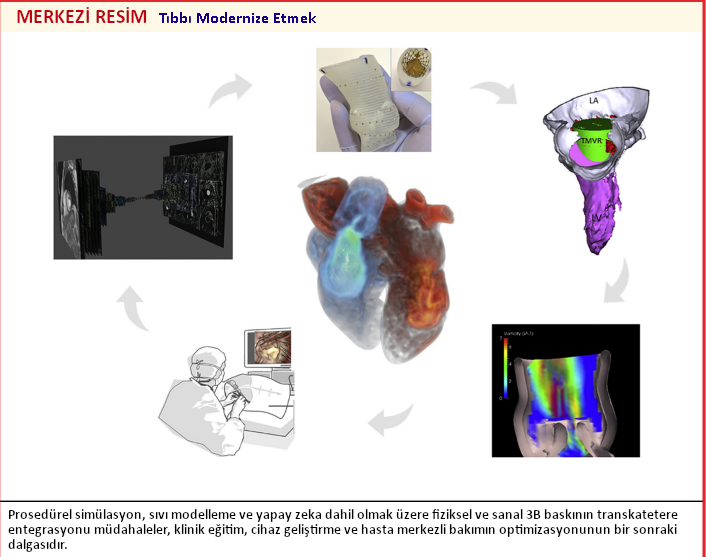
\includegraphics[width=4cm,height=4cm]{Merkezi Resim.png}}
\label{figm}
\end{figure}

\begin{figure}[!t]
\caption{Öne Çıkanlar}
\centerline{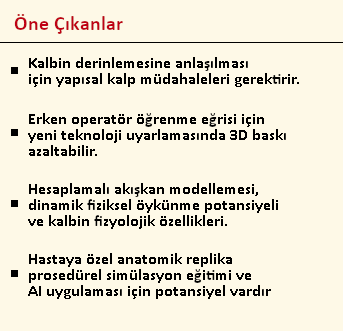
\includegraphics[width=4cm,height=4cm]{Öne Çıkanlar.png}}
\label{figö}
\end{figure}

\begin{figure}[!t]
\caption{3D Yazıcı Teknolojileri}
\centerline{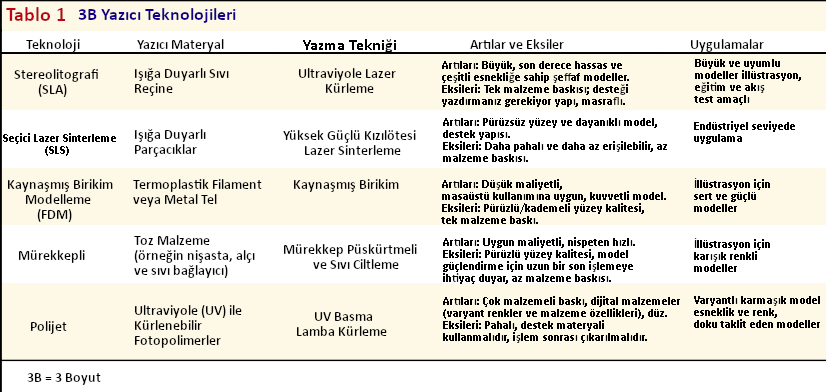
\includegraphics[width=4cm,height=4cm]{Tablo 1.png}}
\label{figt1}
\end{figure}

\begin{figure}[!t]
\caption{3D Baskı İçin Görüntüleme Teknikleri}
\centerline{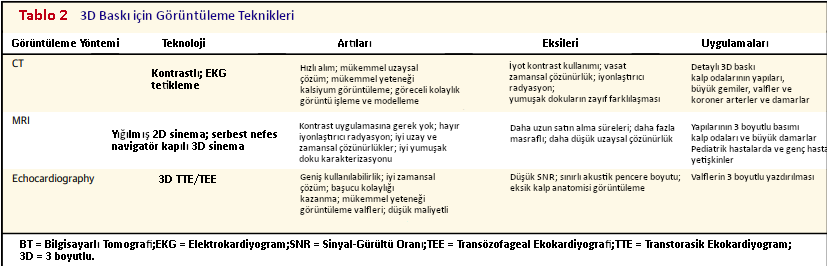
\includegraphics[width=4cm,height=4cm]{Tablo 2.png}}
\label{figt2}
\end{figure}

\end{document}
